%%%%%%%%%%%%%%%%%%%%%%%%%%%%%%%%%%%%%%%%%%%%%%%%%%%%%%%%%%%%%%%%%%%%%%%%%%%%%%%%%%%%
%Do not alter this block of commands.  If you're proficient at LaTeX, you may include additional packages, create macros, etc. immediately below this block of commands, but make sure to NOT alter the header, margin, and comment settings here. 
\documentclass[12pt]{article}
 \usepackage[margin=1in]{geometry} 
\usepackage{amsmath,amsthm,amssymb,amsfonts, enumitem, fancyhdr, color, hyperref,comment, graphicx, environ,mathtools, bbm, tikz, setspace, cleveref,listings, dcolumn}
\usepackage{array, multirow, caption, booktabs}
\usepackage{ mathrsfs }
\usetikzlibrary{matrix,positioning}
\tikzset{bullet/.style={circle,draw=black,inner sep=8pt}}
\DeclareMathOperator*{\argmax}{arg\,max}
\DeclareMathOperator*{\argmin}{arg\,min}
\DeclareMathOperator*{\Var}{\text{Var}}
\DeclareMathOperator*{\Cov}{\text{Cov}}

\DeclarePairedDelimiter\norm{\lVert}{\rVert}%
\newtheorem{theorem}{Theorem}
\newtheorem{lemma}[theorem]{Lemma}
\DeclareMathOperator{\eps}{\varepsilon}

\DeclarePairedDelimiter\abs{\lvert}{\rvert}%
\pagestyle{fancy}
\setlength{\headheight}{65pt}
\newenvironment{problem}[2][Problem]{\begin{trivlist}
\item[\hskip \labelsep {\bfseries #1}\hskip \labelsep {\bfseries #2.}]}{\end{trivlist}}
\newenvironment{sol}
    {\emph{Solution:}
    }
    {
    \qed
    }


%%%%%%%%%%%%%%%%%%%%%%%%%%%%%%%%%%%%%%%%%%%%%%%%%%%%%%%%%%%%%%%%%%%%%%%%%%%%%%%%%


\usepackage{xcolor}
 


%%%%%%%%%%%%%%%%%%%%%%%%%%%%%%%%%%%%%%%%%%%%%

\rhead{John Higgins\\Econ 715 \\ 1 December, 2022} 

%%%%%%%%%%%%%%%%%%%%%%%%%%%%%%%%%%%%%%%%%%%%%


%%%%%%%%%%%%%%%%%%%%%%%%%%%%%%%%%%%%%%

\begin{document}
Note: I used R instead of Matlab and have included a copy of my code in the file PS1b.R! 

\begin{problem}{1}
\end{problem}
\begin{sol}
\begin{enumerate}[label=\alph*) ]
  \item I estimate the OLS model and include the results below:
  \begin{table}[!htbp] \centering 
    \caption{} 
    \label{} 
  \begin{tabular}{@{\extracolsep{5pt}}lc} 
  \\[-1.8ex]\hline 
  \hline \\[-1.8ex] 
   & \multicolumn{1}{c}{\textit{Dependent variable:}} \\ 
  \cline{2-2} 
  \\[-1.8ex] & log\_earn \\ 
  \hline \\[-1.8ex] 
   education & 0.151$^{***}$ \\ 
    & (0.004) \\ 
   exp & 0.059 \\ 
    & (0.066) \\ 
   exp2 & $-$0.002 \\ 
    & (0.003) \\ 
   Constant & 8.036$^{***}$ \\ 
    & (0.377) \\ 
  \hline \\[-1.8ex] 
  Observations & 6,134 \\ 
  R$^{2}$ & 0.181 \\ 
  Adjusted R$^{2}$ & 0.181 \\ 
  Residual Std. Error & 0.550 (df = 6130) \\ 
  F Statistic & 451.979$^{***}$ (df = 3; 6130) \\ 
  \hline 
  \hline \\[-1.8ex] 
  \textit{Note:}  & \multicolumn{1}{r}{$^{*}$p$<$0.1; $^{**}$p$<$0.05; $^{***}$p$<$0.01} \\ 
  \end{tabular} 
  \end{table} 
  \item I run the quantile regression for the $\tau = 0.5 $ and $\tau = 0.75$ quantiles and include the results below:
  \begin{table}[htbp]
    \centering
    \caption{Quantile regression results (bootstrap standard errors)}
      \begin{tabular}{lcccc}
          \toprule
            Coefficient                & Estimate ($\tau = 0.5)$   & SE ($\tau = 0.5)$ &     Estimate ($\tau = 0.75)$   & SE ($\tau = 0.75)$          \\
          \midrule
          Intercept & 8.838$^{***}$ & 0.395 &  8.303$^{***}$ & 0.508\\
          Education & 0.138$^{***}$ & 0.005 & 0.154$^{***}$ & 0.005\\
          Experience & -0.047 & 0.067 & 0.062 & 0.090\\
          Experience$^2$ & 0.003 & 0.003 & -0.002 & 0.004\\
          \bottomrule
      \end{tabular}
    \label{tab:qreg}
  \end{table}
\end{enumerate}
\end{sol}
\begin{problem}{2}
\end{problem}
\begin{sol}
  \begin{enumerate}[label=\alph*) ]
  \item For GMM, we have the following moment condition:
  \[E[((1-\tau) \mathbbm{1}(log(wage_i) \leq \alpha + x_i \beta ) - \tau \mathbbm{1}(log(wage_i) > \alpha + x_i \beta )x_i ] = 0\]
  Equivalently, we can write this as:
  \[E[(\mathbbm{1}(log(wage_i) \leq \alpha + x_i \beta ) - \tau) x_i] = 0\]
  The GMM criterion function (with weight matrix $W_n$) is thus by the following:
\[\left[\frac{1}{n} \sum_{i=1}^n (\mathbbm{1}(log(wage_i) \leq \alpha + x_i \beta ) - \tau) x_i\right]' W_n \left[\frac{1}{n} \sum_{i=1}^n (\mathbbm{1}(log(wage_i) \leq \alpha + x_i \beta ) - \tau) x_i\right]  \]
\item Using the identity matrix as $W_n$, I estimated the regression using GMM for $\tau = 0.5$ and $\tau = 0.75$ and included my coefficient estimates below:
\begin{table}[htbp]
  \centering
  \caption{GMM regression results}
    \begin{tabular}{lcccc}
        \toprule
          Coefficient          & Estimate ($\tau = 0.5)$  &     Estimate ($\tau = 0.75)$           \\
        \midrule
        Intercept & 8.834 &   8.314  \\
        Education & 0.138 & 0.154 \\
        Experience & -0.046 &  0.061  \\
        Experience$^2$ & 0.003 &  -0.002  \\
        \bottomrule
    \end{tabular}
  \label{tab:gmmreg}
\end{table}
\item The asymptotic variance-covariance of the GMM quantile regression coefficient estimators with $\tau = 0.75$ is given by the following:
\[V = (\Gamma' \Omega^{-1} \Gamma)^{-1}\]
where
\[\Omega = (0.75)(0.25)E[x x']\]
and 
\[\Gamma = E[f_{\eps \mid x}(0) x x']\]
We then have that
\[\sqrt(n)(\hat{\beta}_{\tau} - \beta_{\tau}) \rightarrow_d N(0, V)\]
\item Under the assumption that errors are independent of regressors, I estimate the asymptotic variance-covariance matrix to be the following:
\[\hat{V} = \begin{bmatrix}
  1452.73 & -2.76 & -248.98 & 10.72 \\ 
  -2.76 & 0.18 & 0.06 & -0.00 \\ 
  -248.98 & 0.06 & 43.87 & -1.90 \\ 
  10.72 & -0.00 & -1.90 & 0.08 \\ 
  \end{bmatrix}\]
  This leads to the following standard errors:
  \[se(\alpha) = 0.487 \quad se(\beta_1) = 0.005 \quad se(\beta_2) = 0.084 \quad se(\beta_3 ) = 0.004\]
  These roughly align with the standard errors from quantile regression, which is encouraging!

  I also (initially, because I didn't read the question) did the estimation under the assumption that the errors are not independent. I used the Powell estimator with bandwidth $h = 0.01$ (this was arbitrary) to estimate $\Gamma$ and estimated the following covariance matrix:
  \[\hat{V} = \begin{bmatrix}
    2373.04 & -4.86 & -405.39 & 17.44 \\ 
    -4.86 & 0.28 & 0.17 & -0.01 \\ 
    -405.39 & 0.17 & 71.17 & -3.07 \\ 
    17.44 & -0.01 & -3.07 & 0.13 \\ 
    \end{bmatrix} \]
    This yields the following standard errors:
    \[se(\alpha) = 0.622 \quad se(\beta_1) = 0.007 \quad se(\beta_2) = 0.108 \quad se(\beta_3 ) = 0.005\]
    These are also very similar to the quantile regression coefficients.
    \item Using the above (i.e. the variance-covariance under independence), I find that the standard error for $\beta_1^{.75}$ is 0.005. 
\end{enumerate}
\end{sol}
\begin{problem}{3}
\end{problem}
\begin{sol}
  \begin{enumerate}[label=\alph*) ]
  \item I obtained the $\tau = 0.75$ quantile for each cell using the quantile function in $R$.
  \item We now find the asymptotic varaince-covariance of the quantile estimators across all the cells. We first note that a quantile estimator $\hat{q}_{\tau}$ for $q_{\tau}$ will have the following asymptotic distribution:
  \[\sqrt{n}(\hat{q}_{\tau} - q_{\tau}) \rightarrow_d N(0, \frac{\tau(1-\tau)}{f(q_{\tau})})\]
  where $f$ is the density of the response variable. 

  Under the assumption that errors are independent of regressors, it follows that there is zero covariance between the quantile estimators for different cells. If we let $\sigma_{i}^2 = \frac{\tau (1-\tau)}{f_{i,j}(q_{\tau})}$ indicate the variance of the quantile estimator for the $i$-th cell, the asymptotic variance-covariance matrix will be the following:
  \[W = I_n \otimes \begin{bmatrix}\sigma_{1}^2 & \sigma_2^2 & \hdots & \sigma_K^2\end{bmatrix}'\]
  (where $K$ is the total number of cells). Essentially, the variance-covariance is a diagonal matrix with each cell's variance of the quantile estimator on the diagonal.
  \item I compute the asymptotic variance-covariance for use in my regression (I don't report here because that's a lot of cells)
  \item I use the following FGLS estimator:
  \[\beta = (X' W^{-1} X)^{-1} X W^{-1} Y\]
  where $W$ is the variance-covariance matrix of the quantile estimator in each cell (computed previously in part c). Using this estimator, I fit a regression line through the log(wage) quantile values using FGLS to estimate equation 1 and obtain the following results:
  \begin{table}[htbp]
    \centering
    \caption{Minimum distance regression results}
      \begin{tabular}{lcccc}
          \toprule
            Coefficient          & Estimate          \\
          \midrule
          Intercept & 8.004  \\
          Education & 0.155 \\
          Experience & 0.110 \\
          Experience$^2$ & -0.004  \\
          \bottomrule
      \end{tabular}
    \label{tab:mdreg}
  \end{table}
  
  I wasn't sure if we were supposed to aggregate the data and run the regression on 30 data points or if we were supposed to run the regression on the original data with each cell's quantile broadcast to each observation in that cell. I also included results for this specification and include them below:
  \begin{table}[htbp]
    \centering
    \caption{Minimum distance regression results (V2)}
      \begin{tabular}{lcccc}
          \toprule
            Coefficient          & Estimate          \\
          \midrule
          Intercept & 8.247  \\
          Education & 0.151 \\
          Experience & 0.077 \\
          Experience$^2$ & -0.002  \\
          \bottomrule
      \end{tabular}
    \label{tab:mdreg2}
  \end{table}
  \item Given the assumption that errors are independent of regressors, the asymptotic variance-covariance for FGLS will be the following:
  \[V = \sigma^2 (X' W^{-1} X)^{-1}\]
  where $\Var(\eps) = \sigma^2 W$ and $W$ is the variance-covariance matrix of the quantile estimator across the cells (computed previously in part c).
  \item The estimated variance-covariance matrix is computed to be the following:
  \[\hat{V} = \begin{bmatrix}
    107.40 & -0.17 & -18.39 & 0.79 \\ 
    -0.17 & 0.01 & -0.00 & 0.00 \\ 
    -18.39 & -0.00 & 3.23 & -0.14 \\ 
    0.79 & 0.00 & -0.14 & 0.01 \\ 
    \end{bmatrix}\]
  \item The standard errors for the coefficients are the following:
  \[se(\alpha) = 0.345 \quad se(\beta_1) = 0.004 \quad se(\beta_2) = 0.0599 \quad se(\beta_3 ) = 0.0026\]
  These are similar to the previously found standard errors.
\end{enumerate}
\end{sol}
\begin{problem}{4}
\end{problem}
\begin{sol}
  \begin{enumerate}[label=\alph*) ]
    \item Taking a random sample of size 400, I use each of the above methods to estimate $\beta_1$. Furthermore, I find the bagged estimates of each one (by resampling with replacement from the random sample 1000 times). I report my coefficient estimates below:
    \begin{table}[htbp]
      \centering
      \caption{Finite sample $\beta_1^{0.75}$ estimates}
        \begin{tabular}{lcc}
            \toprule
              Method          & $\hat{\beta}_1^{0.75}$  & $\hat{\beta}_1^{0.75}$ (bagged)         \\
            \midrule
            qreg & 0.1439 & 0.1403\\
              GMM & 0.1408 & 0.1384\\
              MD & 0.1328 & 0.1304\\
            \bottomrule
        \end{tabular}
      \label{tab:bagged}
    \end{table}
    We can see that these are slightly different from the estimates from the full sample. This is not unexpected, since we have a much smaller sample. 
    \item We now repeat this procedure $J = 400$ times. For each iteration $j = 1, \ldots, 400$, I draw a random sample of size 400. I then take $B = 400$ bootstrap samples with replacement from this sample and compute the bagged estimates. In the following table, I include each set of coefficient estimates, as well as their standard errors and bias. It seems that quantile regression and GMM tend to give roughly the same point estimate, with GMM affording lower variance. Minimum distance seems to have more bias (and higher standard error) than the other two methods. Comparing the standard estimators with the corresponding bagged estimators, the bagged estimates do perform better. The bias is essentially the same, but the bagged version of each estimator has a lower standard error. The reduction in standard error is most pronounced for minimum distance and less pronounced for GMM. My intuition for why the error is much higher for minimum distance comes down to the fact that the aggregation across each cell creates worse finite-sample performance (since the estimator may not be robust to cells with small numbers of observations). This could likely be mitigated by setting a higher minimum number of observations in each cell. In my approach, I eliminated any cells with only 1 observation so that the fitted normal distribution was non-degenerate, but it is entirely possible that a more stringent threshold would give more stable, precise results. 
    \item \begin{table}[htbp]
      \centering
      \caption{Finite sample $\beta_1^{0.75}$ estimates, $J = 400$ iterations:}
        \begin{tabular}{lcccccc}
            \toprule
              Method          & $\hat{\beta}_1^{0.75}$  & SE & Bias & $\hat{\beta}_1^{0.75}$ (bagged) & SE & Bias        \\
            \midrule
            qreg & 0.1519 & 0.019 & -0.002 &0.1520 & 0.017 &-0.002 \\
              GMM & 0.1517& 0.018& -0.002 &0.1517 & 0.017 & -0.002\\
              MD & 0.1580& 0.027 & 0.004 &0.1582 &0.020 & 0.004 \\
            \bottomrule
        \end{tabular}
      \label{tab:bagged_400}
    \end{table}

    For visual comparison, I provide a histogram of each estimator and their corresponding bagged estimates:
    \begin{center}
      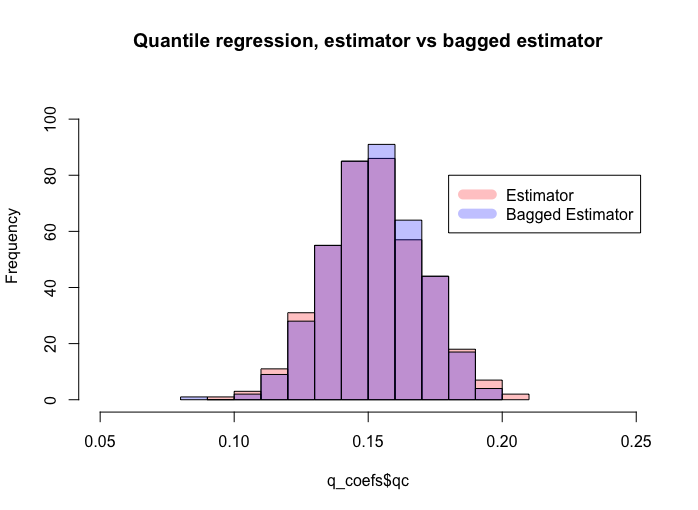
\includegraphics[scale=0.5]{qreg_comp.png}
      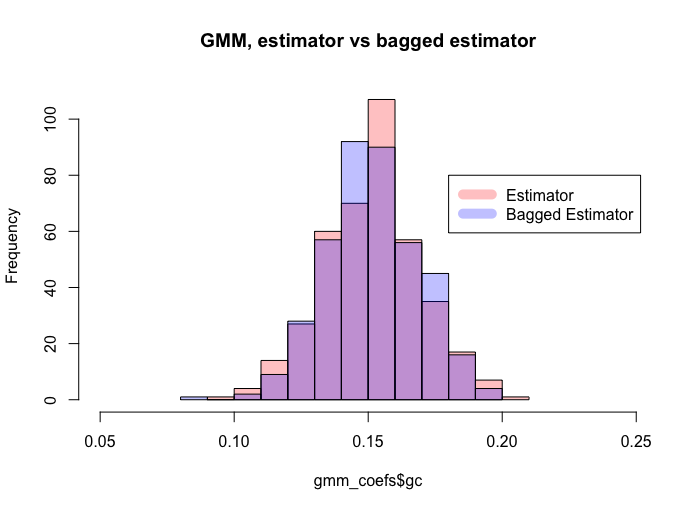
\includegraphics[scale=0.5]{gmm_comp.png}
      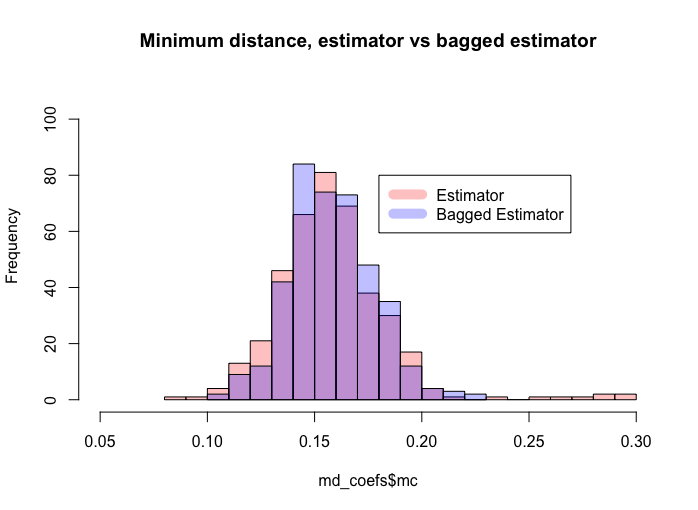
\includegraphics[scale=0.5]{md_comp.png}
    \end{center}
    I also plot the histograms for each type of estimator for comparison. I do the same for the bagged estimates.
    \begin{center}
      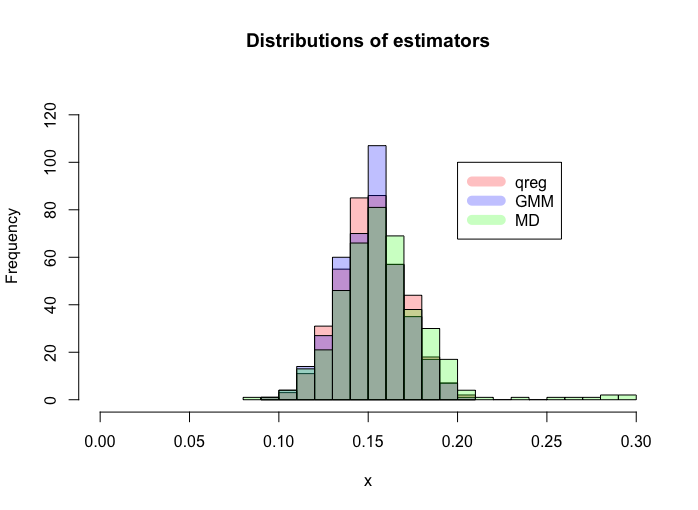
\includegraphics[scale=0.5]{est_comp.png}
      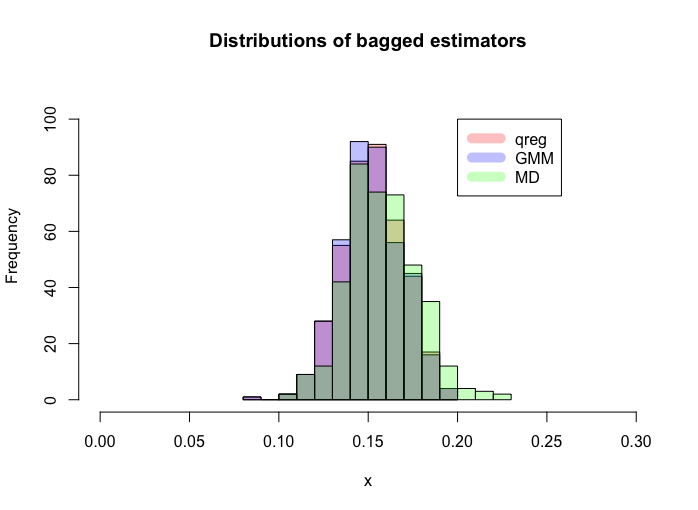
\includegraphics[scale=0.5]{est_comp_bagged.png}
    \end{center}

  \end{enumerate}
\end{sol}

\end{document}
